% Provenance (never printed): see sources/outline_sources.md (Year 3:
% sequence stratigraphy, accommodation and supply, systems tracts,
% cyclostratigraphy). Brief: sources/book5/BRIEFS.md, ch. 16. Curves from
% figdata/bachelor-3/shelf_model.py and lr04_periodogram.py. Exercise and
% problem values in the Book 5 scratch calculator calc/ch16.py. The Varden
% basin, its shelf and its core are invented.
\chapter{Stratigraphie séquentielle}\label{ch:b3:sequence-stratigraphy}

Sur une section sismique d'une marge continentale, les réflecteurs s'appuient en \omterm{def:b3:exploration-seismology:terminations}{onlap} sur les plus anciens,
puis progradent vers le bassin, puis reculent vers la terre, et le motif
se répète plus haut. Chaque ensemble enregistre une lutte entre
deux vitesses~: celle à laquelle la place pour les sédiments se crée, par subsidence et par
la montée de la mer, et celle à laquelle les fleuves la comblent. La stratigraphie séquentielle
lit cette lutte dans la géométrie des couches, et
la \omterm{def:b3:sequence-stratigraphy:cyclo}{cyclostratigraphie} en lit l'horloge dans leur épaisseur.

\begin{recall}
L'espace d'accommodation, l'eustatisme, le niveau marin relatif, la subsidence et le
bassin sédimentaire figurent dans le volume de première année, dans son chapitre sur la diagenèse et les
bassins sédimentaires. Transgression et régression marines ainsi que le cycle eustatique de premier
ordre figurent dans le volume de deuxième année, dans son chapitre sur la Terre phanérozoïque~;
les paramètres de Milankovitch et la précession climatique dans son chapitre sur le
forçage orbital et les âges glaciaires~; le modèle d'âge dans son chapitre sur les archives
climatiques et les proxys. \omterm{def:b3:exploration-seismology:terminations}{Onlap}, \omterm{def:b3:exploration-seismology:terminations}{downlap}, \omterm{def:b3:exploration-seismology:terminations}{toplap}, \omterm{def:b3:exploration-seismology:terminations}{troncature d'érosion} et
\omterm{def:b3:exploration-seismology:seismic-stratigraphy}{stratigraphie sismique} figurent au chapitre~\ref{ch:b3:exploration-seismology}. Les séries de Fourier
et la transformée de Fourier figurent dans les volumes de mathématiques.
\end{recall}

\section{Espace d'accommodation, apport sédimentaire et rivage}\label{sec:b3:sequence-stratigraphy:shoreline}

En tout point d'un bassin, le niveau marin relatif monte au taux $A = \dot E
+ \sigma$, soit le taux eustatique plus le taux de subsidence (une baisse lorsque $A < 0$).
Le niveau marin relatif en un lieu est fixé par le niveau marin global et par
tout ce qui déplace le sol sous lui~: la \omterm{def:b3:lithosphere-thermal-models:thermal-subsidence}{subsidence thermique}, la charge des sédiments et
la flexure qu'elle provoque, le rebond de la croûte après la fonte d'une calotte glaciaire, et
la poussée lente du manteau sous la plaque. La montée du niveau marin relatif crée
de l'espace d'accommodation~; les sédiments le remplissent. Le déplacement du rivage vers le
large ou vers la terre dépend des deux, et non du seul niveau
marin.
% ledger: miller20:rsl

\begin{definition}[Régression normale et régression forcée]\label{def:b3:sequence-stratigraphy:regression}
Une \emph{régression normale}\index{régression normale} est un déplacement du rivage vers le large alors que le
niveau marin relatif monte~: l'apport dépasse
l'espace d'accommodation créé au rivage. Une \emph{régression forcée}\index{régression forcée}
est un déplacement vers le large provoqué par une baisse du niveau marin relatif~: le
rivage est repoussé vers le bassin quel que soit l'apport, et la terre laissée derrière est
exposée et érodée.
\end{definition}

\begin{definition}[Trajectoire du rivage]\label{def:b3:sequence-stratigraphy:trajectory}
La \emph{trajectoire du rivage}\index{trajectoire du rivage} est le chemin suivi par le
rivage au cours du temps, tracé dans une coupe parallèle au pendage et dans le référentiel des
sédiments, de sorte qu'elle montre à la fois le déplacement horizontal du rivage et sa
montée ou sa descente par rapport aux couches sous-jacentes.
\end{definition}

Un profil simple rend la lutte exacte. Derrière le rivage, une plate-forme sommitale plane
de largeur $W$ se trouve au niveau de la mer~; devant elle, une pente frontale d'inclinaison
$\tan\theta$ descend jusqu'au fond du bassin, à une profondeur $D$. L'apport sédimentaire
$Q$ est un volume par unité de temps et par mètre de côte (une surface par unité de temps
dans la coupe).

\begin{proposition}[Trajectoire du rivage]\label{prop:b3:sequence-stratigraphy:trajectory}
Si le niveau marin relatif monte ($A \ge 0$) et que la plate-forme sommitale s'aggrade uniformément,
le rivage se déplace à la vitesse
\[
\frac{\mathrm dx_s}{\mathrm dt} = \frac{Q - AW}{D}~;
\]
il prograde tant que $Q > AW$ et recule lorsque $AW > Q$. Si le niveau marin relatif
baisse ($A < 0$), la plate-forme sommitale ne reçoit rien et
\[
\frac{\mathrm dx_s}{\mathrm dt} = \frac{Q}{D} + \frac{|A|}{\tan\theta}.
\]
Dans les deux cas, la trajectoire monte ou descend selon l'angle dont la tangente vaut
$A/(\mathrm dx_s/\mathrm dt)$.
\end{proposition}

\begin{proof}
Pendant un intervalle $\mathrm dt$, la plate-forme sommitale a besoin de $AW\,\mathrm dt$ de sédiments pour
rester au niveau de la mer. Ce qui reste, soit $(Q - AW)\,\mathrm dt$, s'étale sur la pente frontale,
un mur de hauteur $D$, qui avance de $(Q - AW)\,\mathrm dt/D$~; un reliquat négatif
signifie que la mer inonde la plate-forme plus vite qu'elle ne la comble. Quand la mer
baisse, la plate-forme sommitale est hors de l'eau et ne reçoit rien, et le rivage
glisse le long de l'ancienne pente frontale de $|A|\,\mathrm dt/\tan\theta$ sans
apport de sédiments, tandis que tout l'apport construit la pente vers l'avant de $Q\,\mathrm
dt/D$. Le rivage monte de $A\,\mathrm dt$ par rapport aux couches sous-jacentes
pendant qu'il se déplace de $\mathrm dx_s$, ce qui donne l'angle.
\end{proof}

Une \omterm{def:b3:sequence-stratigraphy:regression}{régression normale} exige donc un apport supérieur à l'espace d'accommodation
créé sur la plate-forme sommitale, et sa trajectoire monte~; une \omterm{def:b3:sequence-stratigraphy:regression}{régression forcée} se produit
quel que soit l'apport, et sa trajectoire descend. Le rapport des deux taux,
souvent noté $A/S$, classe les motifs~: progradation lorsque $A/S < 1$ sur la
plate-forme sommitale, aggradation voisine de 1, rétrogradation au-delà. Une même courbe du niveau marin
peut donc donner une régression sur une marge riche en sédiments et une
transgression sur une marge sous-alimentée.

\section{Géométrie des strates~: séquences et cortèges sédimentaires}\label{sec:b3:sequence-stratigraphy:sequences}

Les terminaisons de réflecteurs du chapitre~\ref{ch:b3:exploration-seismology}
constituent le vocabulaire de la méthode~: l'\omterm{def:b3:exploration-seismology:terminations}{onlap} et le \omterm{def:b3:exploration-seismology:terminations}{downlap} marquent la base d'un
ensemble, le \omterm{def:b3:exploration-seismology:terminations}{toplap} et la \omterm{def:b3:exploration-seismology:terminations}{troncature d'érosion} son sommet. Lues dans une coupe parallèle au pendage, elles
découpent une marge en ensembles bornés par des surfaces de non-dépôt ou
d'érosion, dont chacun enregistre un cycle de niveau marin relatif.

\begin{definition}[Séquence de dépôt et limite de séquence]\label{def:b3:sequence-stratigraphy:sequence}
Une \emph{séquence de dépôt}\index{séquence de dépôt} est une succession
de strates génétiquement liées, sans rupture majeure en son sein, bornée à sa base
et à son sommet par des discordances ou par les concordances qui les prolongent dans le
bassin. Sa surface de bordure est la \emph{limite de
séquence}\index{limite de séquence}~: une discordance creusée par l'exposition et l'érosion sur la
plate-forme pendant une baisse du niveau marin relatif, passant vers le bassin à une
concordance corrélative.
\end{definition}

\begin{definition}[Cortège sédimentaire]\label{def:b3:sequence-stratigraphy:tract}
Un \emph{cortège sédimentaire}\index{cortège sédimentaire} est l'ensemble des systèmes de dépôt
(fluviaux, côtiers, de plate-forme, de talus) qui ont été actifs ensemble pendant une
partie d'un cycle de niveau marin relatif, reconnu à sa position dans la
séquence, à ses surfaces de bordure et à son mode d'empilement. Quatre sont
distingués~:
\begin{itemize}
\item le \emph{cortège de chute}\index{cortège de chute},
  construit par \omterm{def:b3:sequence-stratigraphy:regression}{régression forcée} pendant la baisse du niveau marin relatif~:
  des foresets en marches descendantes, détachés de l'ancienne plate-forme~;
\item le \emph{cortège de bas niveau}\index{cortège de bas niveau},
  construit par \omterm{def:b3:sequence-stratigraphy:regression}{régression normale} dès que le niveau marin relatif recommence à monter,
  à la position la plus basse du rivage~: un prisme en aggradation et en progradation~;
\item le \emph{cortège transgressif}\index{cortège transgressif},
  construit pendant le recul du rivage vers l'intérieur des terres~: des unités en rétrogradation
  en \omterm{def:b3:exploration-seismology:terminations}{onlap} sur l'ancienne plate-forme~;
\item le \emph{cortège de haut niveau}\index{cortège de haut niveau},
  construit par \omterm{def:b3:sequence-stratigraphy:regression}{régression normale} en fin de remontée, lorsque l'apport sédimentaire dépasse de nouveau
  l'espace d'accommodation~: des foresets qui progradent et se terminent en \omterm{def:b3:exploration-seismology:terminations}{downlap} sur les dépôts sous-jacents.
\end{itemize}
\end{definition}

\begin{definition}[Surfaces de transgression et d'inondation maximale]\label{def:b3:sequence-stratigraphy:surfaces}
La \emph{surface de transgression}\index{surface de transgression} est la première
\omterm{def:b3:sequence-stratigraphy:parasequence}{surface d'inondation} significative au-dessus des dépôts de bas niveau~: elle marque le passage
du rivage de la régression à la transgression. La \emph{surface d'inondation
maximale}\index{surface d'inondation maximale} marque la position la plus en retrait du
rivage, le passage de la transgression à la régression de haut niveau~; les
foresets de haut niveau se terminent en \omterm{def:b3:exploration-seismology:terminations}{downlap} sur elle.
\end{definition}

\begin{definition}[Section condensée et vallée incisée]\label{def:b3:sequence-stratigraphy:condensed}
Une \emph{section condensée}\index{section condensée} est un intervalle mince
déposé très lentement loin du rivage, pendant que la mer envahit la plate-forme
et que les sédiments sont piégés près de la côte~: quelques centimètres ou décimètres
d'argile, de fossiles, de glauconie ou de phosphate, qui peuvent enregistrer un long laps de temps. Une
\emph{vallée incisée}\index{vallée incisée} est une vallée fluviale creusée dans la
plate-forme exposée pendant la baisse du niveau marin relatif, et comblée pendant le
bas niveau et la transgression qui suivent.
\end{definition}

\begin{omfigure}
\begin{tikzpicture}[font=\scriptsize, x=0.9cm, y=1.25cm, >=Stealth]
% older highstand deposits below the sequence boundary
\fill[black!10] (0,0) -- (14,0) -- (14,0.4) -- (10,0.6) -- (6,2.8) -- (0,3.0) -- cycle;
\draw[black!35] (1.5,2.0) .. controls (3.2,1.95) and (4.5,1.2) .. (8.5,0.45);
\draw[black!35] (3.5,2.93) .. controls (4.8,2.85) and (6,1.6) .. (10.5,0.42);
% falling-stage systems tract
\fill[red!25] (6.0,2.8) -- (7.4,2.25) -- (8.4,1.85) -- (9.4,1.35) -- (10.4,0.75) -- (10.6,0.58) -- (10,0.6) -- cycle;
\draw[red!60!black] (6.6,2.56) .. controls (7.0,2.4) and (7.5,1.95) .. (8.0,1.70);
\draw[red!60!black] (7.6,2.17) .. controls (8.0,2.0) and (8.5,1.45) .. (9.0,1.15);
\draw[red!60!black] (8.6,1.75) .. controls (9.0,1.55) and (9.5,0.9) .. (10.0,0.6);
% lowstand wedge
\fill[orange!40] (9.2,1.45) -- (10.4,1.5) -- (11.5,1.0) -- (12.6,0.6) -- (13.4,0.44) -- (10.6,0.58) -- (10.4,0.75) -- cycle;
% incised valley and its fill
\fill[orange!30] (2.9,2.9) .. controls (3.3,2.3) and (3.9,2.3) .. (4.3,2.86) -- cycle;
% transgressive systems tract
\fill[green!45!black!35] (11.5,1.0) -- (10.4,1.5) -- (9.2,1.45) -- (8.4,1.85) -- (7.4,2.25) -- (6.0,2.8) -- (1.0,2.97) -- (1.0,3.05) -- (6.0,2.95) -- (7.6,2.5) -- (9.4,1.75) -- (10.8,1.45) -- cycle;
% highstand systems tract
\fill[blue!22] (0,3.62) -- (7.5,3.42) -- (9.8,2.2) -- (11.2,1.22) -- (10.8,1.45) -- (9.4,1.75) -- (7.6,2.5) -- (6.0,2.95) -- (1.0,3.05) -- (0,3.07) -- cycle;
\draw[blue!60!black] (4.0,3.52) .. controls (5.0,3.45) and (5.8,3.1) .. (6.6,2.79);
\draw[blue!60!black] (5.6,3.47) .. controls (6.6,3.4) and (7.4,2.8) .. (8.2,2.26);
\draw[blue!60!black] (6.8,3.44) .. controls (7.8,3.35) and (8.8,2.4) .. (9.7,1.69);
% surfaces
\draw[red!70!black, very thick] (0,3.0) -- (2.9,2.9) .. controls (3.3,2.3) and (3.9,2.3) .. (4.3,2.86) -- (6.0,2.8) -- (7.4,2.25) -- (8.4,1.85) -- (9.2,1.45);
\draw[red!70!black, very thick, densely dashed] (9.2,1.45) -- (9.4,1.35) -- (10.4,0.75) -- (10.6,0.58) -- (14,0.4);
\draw[green!40!black, thick] (11.5,1.0) -- (10.4,1.5) -- (9.2,1.45);
\draw[blue!60!black, thick] (0,3.07) -- (1.0,3.05) -- (6.0,2.95) -- (7.6,2.5) -- (9.4,1.75) -- (10.8,1.45) -- (11.5,1.03) -- (12.6,0.63) -- (13.4,0.47) -- (14,0.43);
% labels
\node[blue!50!black] at (2.6,3.36) {haut niveau (HST)};
\node[green!35!black, anchor=south] at (4.8,3.92) {transgressif (TST)};
\draw[green!35!black] (4.8,3.92) -- (4.4,3.01);
\node[red!60!black, anchor=west] at (10.1,2.45) {chute (FSST)};
\draw[red!60!black] (10.1,2.45) -- (8.8,1.62);
\node[orange!60!black, anchor=west] at (12.2,1.55) {bas niveau (LST)};
\draw[orange!60!black] (12.2,1.55) -- (11.2,0.85);
\node[anchor=north, align=center] at (3.6,2.25) {vallée\\ incisée};
\node[red!70!black, anchor=north] at (1.4,2.95) {SB};
\node[red!70!black, anchor=north] at (12.0,0.38) {concordance corrélative};
\node[blue!60!black, anchor=west] at (12.7,1.1) {MFS};
\draw[blue!60!black] (12.7,1.1) -- (12.1,0.82);
\node[green!40!black, anchor=west] at (11.6,2.0) {TS};
\draw[green!40!black] (11.6,2.0) -- (10.9,1.27);
\node[blue!60!black, anchor=south] at (13.4,0.58) {condensée};
\node[anchor=west, black!60] at (0.2,0.35) {dépôts plus anciens};
\draw[->] (11.2,3.9) -- (12.6,3.9) node[right] {vers le bassin};
\end{tikzpicture}

\par\smallskip{\small Anatomie d'une \omterm{def:b3:sequence-stratigraphy:sequence}{séquence de dépôt} en coupe dans le sens du pendage
(schématique, échelle verticale très exagérée). La \omterm{def:b3:sequence-stratigraphy:sequence}{limite de séquence} (SB, en rouge)
est une discordance sur la plate-forme, avec une \omterm{def:b3:sequence-stratigraphy:condensed}{vallée incisée}, et une
concordance corrélative dans le bassin (en pointillés)~; ici elle est tracée au-dessus des
dépôts de chute. La \omterm{def:b3:sequence-stratigraphy:surfaces}{surface de transgression} (TS) coiffe le prisme de bas niveau~; la \omterm{def:b3:sequence-stratigraphy:surfaces}{surface d'inondation
maximale} (MFS) coiffe le \omterm{def:b3:sequence-stratigraphy:tract}{cortège transgressif} mince et passe vers le bassin
à une \omterm{def:b3:sequence-stratigraphy:condensed}{section condensée}~; les foresets de haut niveau se terminent en \omterm{def:b3:exploration-seismology:terminations}{downlap} sur elle.}\label{fig:b3:sequence-stratigraphy:anatomy}
\end{omfigure}

Le tracé exact de la \omterm{def:b3:sequence-stratigraphy:sequence}{limite de séquence} dans le bassin relève d'une convention, et
les auteurs ne sont pas d'accord~: certains la placent à la base des dépôts de chute, là où
la baisse commence, d'autres à leur sommet, là où elle se termine, comme dans la figure ci-dessus.
Sur la plate-forme, il n'y a pas d'ambiguïté~: la limite est la surface d'exposition
et d'érosion, et les dépôts qui la surmontent sont postérieurs à la baisse.

Lue de bas en haut en un point de la plate-forme externe, une séquence enregistre
le cycle~: foresets de haut niveau, une surface d'exposition, peut-être un remplissage de vallée,
la \omterm{def:b3:sequence-stratigraphy:surfaces}{surface de transgression}, des bancs en rétrogradation, un intervalle condensé à la
\omterm{def:b3:sequence-stratigraphy:surfaces}{surface d'inondation maximale}, puis de nouveau des foresets de haut niveau. La hiérarchie des
cycles est fixée par leurs causes~: l'ouverture et la fermeture des océans pour le
cycle de premier ordre, les variations du volume des glaces et de la vitesse d'expansion des fonds
océaniques pour les plus courts, et la tectonique locale et l'apport sédimentaire pour l'ensemble
d'entre eux.

\section{Paraséquences et motifs d'empilement}\label{sec:b3:sequence-stratigraphy:parasequences}

À l'intérieur d'un \omterm{def:b3:sequence-stratigraphy:tract}{cortège sédimentaire}, les plus petits ensembles qu'un géologue cartographie sur une falaise ou sur une diagraphie de puits
sont des unités dont la profondeur diminue vers le haut, épaisses de quelques mètres à quelques dizaines de mètres,
coiffées par une surface où une eau plus profonde revient brusquement.

\begin{definition}[Paraséquence et surface d'inondation]\label{def:b3:sequence-stratigraphy:parasequence}
Une \emph{paraséquence}\index{paraséquence} est une succession relativement concordante de bancs génétiquement liés,
bornée par des surfaces d'inondation, dans laquelle l'eau devient moins profonde vers le haut~: sur une côte dominée par les vagues,
les boues du large passent vers le haut aux sables de l'avant-côte inférieur et supérieur, puis à la plage. Une
\emph{surface d'inondation}\index{surface d'inondation} est une surface sur laquelle des faciès de plus grande profondeur
recouvrent brutalement des faciès moins profonds,
avec des indices d'un approfondissement soudain.
\end{definition}

Une \omterm{def:b3:sequence-stratigraphy:parasequence}{paraséquence} isolée devient plus grossière vers le haut, et sa diagraphie gamma, pauvre en sable
et riche en argile, dessine une forme d'entonnoir qui se resserre vers le haut. La manière dont les
\omterm{def:b3:sequence-stratigraphy:parasequence}{paraséquences} d'un même cortège s'empilent les unes sur les autres renseigne sur la tendance du rivage~:
chacune se construit plus loin vers le large que la précédente (progradation),
au-dessus de la précédente (aggradation), ou en retrait vers la terre (rétrogradation). Une diagraphie
qui traverse l'empilement montre directement cette tendance~: chaque \omterm{def:b3:sequence-stratigraphy:parasequence}{paraséquence} se termine par des faciès plus grossiers
et moins profonds que celui du dessous, identiques, ou plus fins et plus profonds.
Les \omterm{def:b3:sequence-stratigraphy:tract}{cortèges de haut niveau} et de bas niveau s'empilent par progradation ou par aggradation,
les \omterm{def:b3:sequence-stratigraphy:tract}{cortèges transgressifs} par rétrogradation. Le chapitre suivant lit
ces diagraphies faciès par faciès.

\begin{omfigure}
\begin{tikzpicture}[font=\scriptsize, x=1cm, y=1cm]
% three logs: each parasequence a coarsening-upward wedge (grain size to the right)
% progradational
\begin{scope}[xshift=0cm]
\fill[yellow!45!brown!35] (0,0) -- (0.5,0) -- (1.4,1.1) -- (0,1.1) -- cycle;
\fill[yellow!45!brown!35] (0,1.1) -- (0.5,1.1) -- (1.8,2.2) -- (0,2.2) -- cycle;
\fill[yellow!45!brown!35] (0,2.2) -- (0.5,2.2) -- (2.2,3.3) -- (0,3.3) -- cycle;
\draw (0,0) -- (0.5,0) -- (1.4,1.1) -- (0.5,1.1) -- (1.8,2.2) -- (0.5,2.2) -- (2.2,3.3) -- (0,3.3) -- cycle;
\node[anchor=north, align=center] at (1.1,-0.1) {progradation\\ (le rivage se déplace vers le large)};
\end{scope}
% aggradational
\begin{scope}[xshift=4.2cm]
\fill[yellow!45!brown!35] (0,0) -- (0.5,0) -- (1.8,1.1) -- (0,1.1) -- cycle;
\fill[yellow!45!brown!35] (0,1.1) -- (0.5,1.1) -- (1.8,2.2) -- (0,2.2) -- cycle;
\fill[yellow!45!brown!35] (0,2.2) -- (0.5,2.2) -- (1.8,3.3) -- (0,3.3) -- cycle;
\draw (0,0) -- (0.5,0) -- (1.8,1.1) -- (0.5,1.1) -- (1.8,2.2) -- (0.5,2.2) -- (1.8,3.3) -- (0,3.3) -- cycle;
\node[anchor=north, align=center] at (1.1,-0.1) {aggradation\\ (le rivage reste fixe)};
\end{scope}
% retrogradational
\begin{scope}[xshift=8.4cm]
\fill[yellow!45!brown!35] (0,0) -- (0.5,0) -- (2.2,1.1) -- (0,1.1) -- cycle;
\fill[yellow!45!brown!35] (0,1.1) -- (0.5,1.1) -- (1.8,2.2) -- (0,2.2) -- cycle;
\fill[yellow!45!brown!35] (0,2.2) -- (0.5,2.2) -- (1.4,3.3) -- (0,3.3) -- cycle;
\draw (0,0) -- (0.5,0) -- (2.2,1.1) -- (0.5,1.1) -- (1.8,2.2) -- (0.5,2.2) -- (1.4,3.3) -- (0,3.3) -- cycle;
\node[anchor=north, align=center] at (1.1,-0.1) {rétrogradation\\ (le rivage se déplace vers la terre)};
\end{scope}
% flooding surfaces
\foreach \s in {0,4.2,8.4} {
  \draw[omDef, thick] (\s-0.15,1.1) -- (\s+2.5,1.1);
  \draw[omDef, thick] (\s-0.15,2.2) -- (\s+2.5,2.2);
  \node[omDef, anchor=west] at (\s+2.5,1.1) {SI};
  \node[omDef, anchor=west] at (\s+2.5,2.2) {SI};
}
% grain-size axis
\draw[->] (0,3.6) -- (2.3,3.6) node[right] {plus grossier};
\node[anchor=east] at (0,3.6) {boue};
\end{tikzpicture}

\par\smallskip{\small Trois \omterm{def:b3:sequence-stratigraphy:parasequence}{paraséquences} empilées de trois façons, représentées sous forme de
profils granulométriques (une largeur vers la droite signifie un grain plus grossier). Chaque \omterm{def:b3:sequence-stratigraphy:parasequence}{paraséquence}
devient plus grossière vers le haut, des boues du large aux sables d'avant-côte, et se termine par une
\omterm{def:b3:sequence-stratigraphy:parasequence}{surface d'inondation} (SI)~; le sommet de chacune est plus grossier que celui du dessous lorsque l'empilement
prograde, identique lorsqu'il aggrade, plus fin lorsqu'il
rétrograde.}\label{fig:b3:sequence-stratigraphy:stacking}
\end{omfigure}

\begin{inthefield}[Paraséquences dans une falaise désertique]
\begin{minipage}[t]{0.52\linewidth}\vspace{0pt}
Les Book Cliffs, dans l'est de l'Utah, exposent des dépôts de rivage du Crétacé supérieur
sur des dizaines de kilomètres. Dans le membre de Kenilworth, suivi le long des falaises
de Price à Hatch Mesa, les géologues ont cartographié des dépôts de plaine côtière, d'avant-côte,
de plate-forme interne et de \omterm{def:b3:sequence-stratigraphy:condensed}{vallée incisée}, et neuf \omterm{def:b3:sequence-stratigraphy:parasequence}{paraséquences} à grossissement vers le haut,
dominées par les vagues à la tempête, épaisses de 7 à \qty{32}{m}. Vers le bassin,
chacune se divise en au plus quatre petits ensembles de bancs à grossissement vers le haut, épais de 2 à
\qty{18}{m}~; certains sables d'avant-côte reposent sur une base nette, que l'étude
interprète comme des dépôts de bas niveau.
\end{minipage}\hfill
\begin{minipage}[t]{0.44\linewidth}\vspace{0pt}
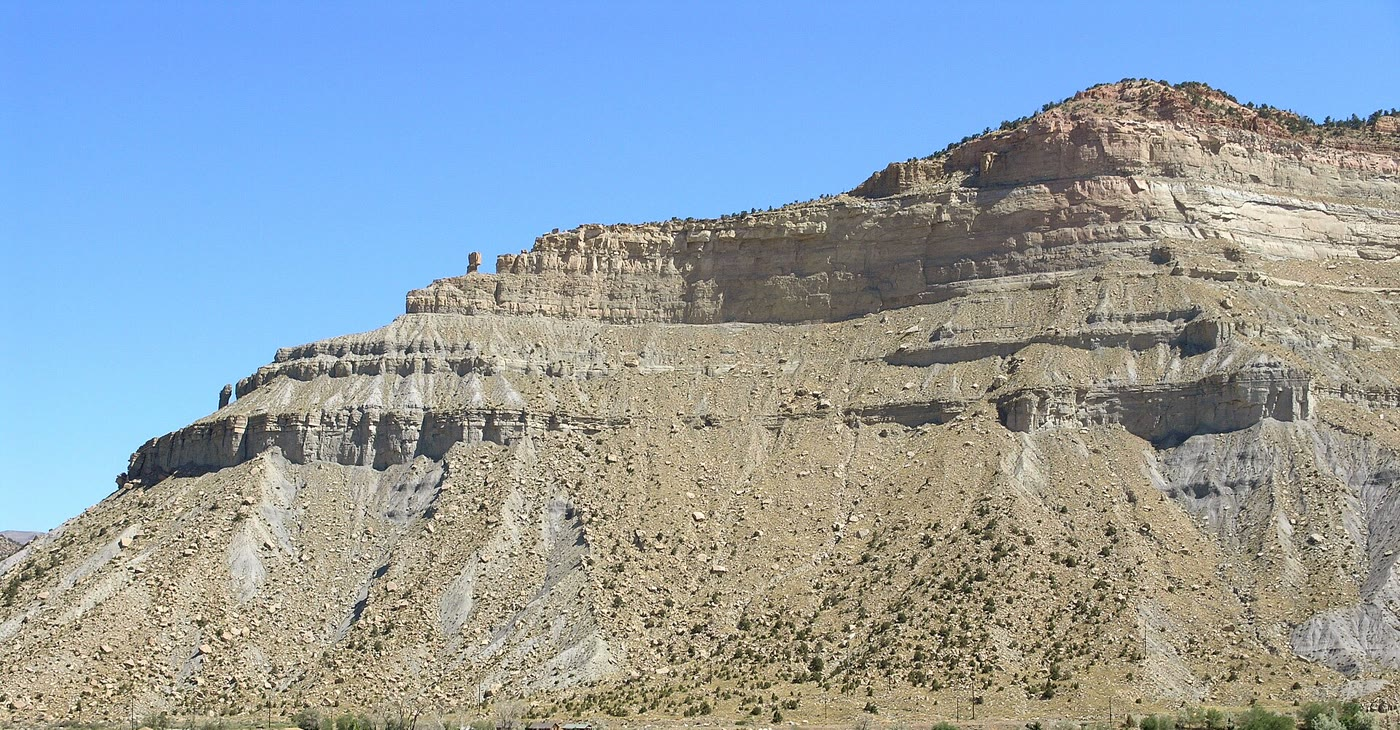
\includegraphics[width=\linewidth]{images/book5/b3-book-cliffs-helper.jpg}

{\scriptsize Les Book Cliffs au-dessus de Helper, Utah~: des corniches de grès pâle se détachent
au-dessus de pentes d'argilite grise. Photo David Mackie, domaine public.}
\end{minipage}
\end{inthefield}
% ledger: pattison95:kenilworth, photo:b3-book-cliffs

\section{Un modèle direct de plate-forme}\label{sec:b3:sequence-stratigraphy:model}

Les règles des sections précédentes peuvent être mises en œuvre sous forme de modèle. Le bassin de Varden
est une plate-forme fictive~: une rampe inclinée vers le bassin à \qty{1.5}{m/km}, subsidant
à $\sigma = 0.02 + x/1200$ \unit{m/ka} à une distance $x$ (km) de la
charnière, sous un niveau marin $E = -30\cos(2\pi t/400)$ (m, $t$ en ka), alimenté par un fleuve
apportant $Q = \qty{6000}{m^3/ka}$ par mètre de côte. À chaque
pas de cinq cents ans, le bassin subside~; les sédiments comblent alors un
topset plat jusqu'au niveau de la mer, là où l'ancienne surface est sous l'eau, et un
foreset de pente 0.012 à l'avant de celui-ci, la position du rivage étant fixée de telle sorte que le volume ajouté
égale l'apport~; les terres émergées ne reçoivent rien et, par souci de
simplicité, ne sont pas érodées. Le modèle part d'un bas niveau, après un premier
prisme sédimentaire construit à niveau marin constant.

\begin{omfigure}
\begin{tikzpicture}
\begin{groupplot}[group style={group size=1 by 2, vertical sep=0.35cm, x descriptions at=edge bottom},
  omrecord, width=0.86\linewidth, xmin=0, xmax=600,
  xtick={0,100,200,300,400,500,600},
  tick label style={font=\scriptsize}, label style={font=\small}]
\nextgroupplot[height=0.2\linewidth, ylabel={$E$ (m)}, ymin=-35, ymax=35,
  ytick={-30,0,30}]
\addplot[omDef, thick, domain=0:600, samples=121] {-30*cos(deg(2*pi*x/400))};
\nextgroupplot[height=0.3\linewidth, xlabel={temps (ka)}, ylabel={rivage $x_s$ (km)},
  ymin=0, ymax=60, ytick={0,20,40,60},
  scatter/classes={1={mark=*, red!70!black}, 2={mark=*, orange!80!black},
    3={mark=*, green!50!black}, 4={mark=*, blue!70!black}}]
% computed in figdata/bachelor-3/shelf_model.py
\addplot[scatter, only marks, mark size=0.9pt, scatter src=explicit symbolic]
  table[x=t, y=xs, meta=tract] {figdata/out/bachelor-3-shelf_model-shore.dat};
\node[font=\scriptsize, orange!60!black] at (axis cs:12,56) {CB};
\node[font=\scriptsize, green!40!black] at (axis cs:70,40) {CT};
\node[font=\scriptsize, blue!60!black] at (axis cs:160,6) {CHN};
\node[font=\scriptsize, red!60!black] at (axis cs:300,22) {CC};
\node[font=\scriptsize, orange!60!black] at (axis cs:415,57) {CB};
\node[font=\scriptsize, green!40!black] at (axis cs:520,45) {CT};
\node[font=\scriptsize, blue!60!black] at (axis cs:580,12) {CHN};
\end{groupplot}
\end{tikzpicture}

\par\smallskip{\small Ci-dessus, le niveau marin eustatique du modèle de Varden~;
ci-dessous, la position du rivage, colorée par \omterm{def:b3:sequence-stratigraphy:tract}{cortège sédimentaire} (bas niveau
orange, transgressif vert, haut niveau bleu, chute rouge), classée
à partir des seules sorties du modèle~: chute lorsque le niveau marin relatif baisse
au rivage, transgressif lorsque le rivage recule, bas niveau ou
haut niveau lorsqu'il avance sous une mer montante, après une chute ou après une
transgression.}\label{fig:b3:sequence-stratigraphy:series}
\end{omfigure}

La figure ci-dessus suit le rivage au fil du temps, et celle ci-dessous
montre les dépôts qu'il a laissés. Les cortèges apparaissent sans qu'aucune règle
ne soit inscrite dans le modèle, hormis le remplissage et la subsidence. Le prisme de bas niveau du début se situe loin
au large~; la mer montante pousse le rivage de \qty{38}{km} vers la terre lors de la
première transgression, et les foresets de haut niveau reprogradent à nouveau à mesure que la remontée ralentit.
Puis la chute commence~: le rivage est repoussé vers le bassin de \qty{33}{km} en
\qty{187}{ka}, laissant de minces foresets en escalier et un plateau
exposé derrière lui, le \omterm{def:b3:sequence-stratigraphy:tract}{cortège de chute}. Un nouveau prisme de bas niveau, une seconde transgression
et un nouveau haut niveau suivent. La vitesse de la \omterm{def:b3:sequence-stratigraphy:regression}{régression forcée} dans le modèle
correspond à la formule de la proposition à quelques pour cent près~; sous une
mer montante, le topset du modèle ne s'aggrade pas uniformément, car la subsidence
croît vers le bassin, et la formule n'est qu'un guide.

\begin{omfigure}
\begin{tikzpicture}
\begin{axis}[omsection, width=0.95\linewidth, height=0.42\linewidth,
  xmin=0, xmax=70, ymin=-150, ymax=40, clip=true,
  xlabel={distance vers le bassin (km)}, ylabel={altitude actuelle (m)},
  xtick={0,10,20,30,40,50,60,70}, ytick={-150,-100,-50,0},
  tick label style={font=\scriptsize}, label style={font=\small}]
% computed in figdata/bachelor-3/shelf_model.py
\addplot[fill=black!10, draw=none] table[x=x, y=z0] {figdata/out/bachelor-3-shelf_model-surfaces.dat} -- (axis cs:120,-300) -- (axis cs:0,-300) -- cycle;
\addplot[fill=orange!45, draw=none] table[x=x, y=z] {figdata/out/bachelor-3-shelf_model-poly1.dat};
\addplot[fill=green!45!black!35, draw=none] table[x=x, y=z] {figdata/out/bachelor-3-shelf_model-poly2.dat};
\addplot[fill=blue!25, draw=none] table[x=x, y=z] {figdata/out/bachelor-3-shelf_model-poly3.dat};
\addplot[fill=red!30, draw=none] table[x=x, y=z] {figdata/out/bachelor-3-shelf_model-poly4.dat};
\addplot[fill=orange!45, draw=none] table[x=x, y=z] {figdata/out/bachelor-3-shelf_model-poly5.dat};
\addplot[fill=green!45!black!35, draw=none] table[x=x, y=z] {figdata/out/bachelor-3-shelf_model-poly6.dat};
\addplot[fill=blue!25, draw=none] table[x=x, y=z] {figdata/out/bachelor-3-shelf_model-poly7.dat};
\addplot[black!45, very thin] table[x=x, y=z40] {figdata/out/bachelor-3-shelf_model-surfaces.dat};
\addplot[black!45, very thin] table[x=x, y=z80] {figdata/out/bachelor-3-shelf_model-surfaces.dat};
\addplot[black!45, very thin] table[x=x, y=z120] {figdata/out/bachelor-3-shelf_model-surfaces.dat};
\addplot[black!45, very thin] table[x=x, y=z160] {figdata/out/bachelor-3-shelf_model-surfaces.dat};
\addplot[black!45, very thin] table[x=x, y=z240] {figdata/out/bachelor-3-shelf_model-surfaces.dat};
\addplot[black!45, very thin] table[x=x, y=z280] {figdata/out/bachelor-3-shelf_model-surfaces.dat};
\addplot[black!45, very thin] table[x=x, y=z320] {figdata/out/bachelor-3-shelf_model-surfaces.dat};
\addplot[black!45, very thin] table[x=x, y=z360] {figdata/out/bachelor-3-shelf_model-surfaces.dat};
\addplot[black!45, very thin] table[x=x, y=z440] {figdata/out/bachelor-3-shelf_model-surfaces.dat};
\addplot[black!45, very thin] table[x=x, y=z480] {figdata/out/bachelor-3-shelf_model-surfaces.dat};
\addplot[black!45, very thin] table[x=x, y=z520] {figdata/out/bachelor-3-shelf_model-surfaces.dat};
\addplot[black!45, very thin] table[x=x, y=z560] {figdata/out/bachelor-3-shelf_model-surfaces.dat};
\addplot[black, thin] table[x=x, y=z600] {figdata/out/bachelor-3-shelf_model-surfaces.dat};
\addplot[black, only marks, mark=*, mark size=0.5pt] table[x=xs, y=zfinal] {figdata/out/bachelor-3-shelf_model-shore.dat};
\node[font=\scriptsize, blue!50!black] at (axis cs:6,4) {CHN};
\node[font=\scriptsize, green!30!black] at (axis cs:12,-22) {CT};
\node[font=\scriptsize, red!60!black] at (axis cs:35,-25) {CC};
\node[font=\scriptsize, orange!60!black] at (axis cs:57.5,-60) {CB};
\node[font=\scriptsize, green!30!black] at (axis cs:36,2) {CT};
\node[font=\scriptsize, blue!50!black] at (axis cs:8,26) {CHN};
\end{axis}
\end{tikzpicture}

\par\smallskip{\small La plate-forme de Varden après \qty{600}{ka}, dans sa position actuelle
(échelle verticale exagérée environ 170 fois). Les couleurs sont les
\omterm{def:b3:sequence-stratigraphy:tract}{cortèges sédimentaires}~: bas niveau orange, transgressif vert, haut niveau bleu,
chute rouge~; le gris figure la rampe plus ancienne et le premier prisme. Les traits fins sont
le fond marin tous les \qty{40}{ka}~; les points noirs suivent le rivage tous les
\qty{2}{ka}. Calculé par le modèle direct décrit
dans le texte.}\label{fig:b3:sequence-stratigraphy:section}
\end{omfigure}


Le niveau marin relatif commence à baisser au rivage quelques milliers d'années
après le haut niveau eustatique, car la subsidence doit d'abord être compensée,
et il cesse de baisser quelques milliers d'années avant le bas niveau eustatique. La chute
au rivage dure donc moins de la moitié du cycle eustatique, et d'autant moins que
le bassin s'enfonce plus vite.

Les modèles de ce type sont le test honnête d'une interprétation, et montrent aussi
ses limites. Une même coupe peut être construite à partir d'histoires différentes~:
une chute plus rapide avec moins d'apport, ou une chute plus lente avec davantage d'apport,
ou un changement de subsidence plutôt que du niveau marin, puisque la géométrie
n'enregistre que le niveau marin relatif et l'apport. Les chartes globales des cycles
du niveau marin, établies à partir de marges dans les années 1970 et 1980, ont fixé le
calendrier de nombreuses chutes que les forages ont depuis largement confirmées pour
certaines parties du Crétacé supérieur au Miocène, mais leurs amplitudes, comme une
chute de \qty{160}{m} à l'Oligocène moyen, sont trop fortes d'un facteur 2 à 3. Les amplitudes
eustatiques se déduisent désormais des isotopes de l'oxygène et de puits décompactés
(backstripping), et les séquences d'une marge se lisent d'abord comme un enregistrement local.
% ledger: miller20:epr, miller20:rsl

\section{Cyclostratigraphie}\label{sec:b3:sequence-stratigraphy:cyclo}

De nombreuses successions se répètent à intervalles d'épaisseur réguliers~: couplets
de marne et de calcaire, paquets de cinq couplets, ensembles plus vastes de paquets. Si
la répétition est rythmée par les paramètres de Milankovitch, l'épaisseur des
cycles se convertit en temps.

\begin{definition}[Cyclostratigraphie et calage astronomique]\label{def:b3:sequence-stratigraphy:cyclo}
La \emph{cyclostratigraphie}\index{cyclostratigraphie} identifie et mesure
des cycles réguliers dans les successions sédimentaires et les interprète comme des enregistrements
d'un forçage périodique, principalement les variations de l'orbite terrestre et de l'axe.
Le \emph{calage astronomique}\index{calage astronomique} attribue des âges à une
succession en faisant correspondre ses cycles, un à un, à une
série astronomique calculée (excentricité, obliquité, précession ou insolation), ce qui transforme les
cycles en modèle d'âge.
\end{definition}

Les périodes calculées proviennent de la solution du mouvement du Système solaire.
L'excentricité de l'orbite terrestre présente un terme principal de \qty{405}{ka}, et
quatre termes voisins de \qty{100}{ka} (95, 99, 124 et \qty{131}{ka})~;
l'obliquité présente un terme principal de \qty{41.0}{ka}, avec des termes plus faibles à 39.6 et
\qty{53.7}{ka}. La précession climatique combine la précession de l'axe
avec le mouvement du périhélie, aux fréquences $p_0 + g_i$, où $p_0 =
50.47''$ par an et les $g_i$ sont des fréquences des orbites planétaires~; ses
périodes principales sont 23.7, 22.4, 19.1 et \qty{19.0}{ka}. Le terme à \qty{405}{ka}
est le plus stable, et sert de métronome aux successions plus anciennes.
% ledger: la04:eccentricity, la04:obliquity, la04:precession

\begin{omfigure}
\begin{tikzpicture}
\begin{groupplot}[group style={group size=2 by 1, horizontal sep=0.5cm, y descriptions at=edge left},
  omrecord, width=0.52\linewidth, height=0.33\linewidth,
  xmin=0, xmax=0.06, ymin=0, ymax=1.18, clip=false,
  xtick={0,0.02,0.04,0.06}, xticklabels={0,0.02,0.04,0.06}, scaled x ticks=false,
  ytick={0,0.5,1}, title style={font=\small},
  tick label style={font=\scriptsize}, label style={font=\small},
  xlabel={fréquence (cycles par ka)}]
\nextgroupplot[title={(a) 0 à \qty{1000}{ka}}, ylabel={puissance relative}]
\draw[black!40, densely dotted] (axis cs:0.01,0) -- (axis cs:0.01,1.05);
\draw[black!40, densely dotted] (axis cs:0.0244,0) -- (axis cs:0.0244,1.05);
\draw[black!40, densely dotted] (axis cs:0.0429,0) -- (axis cs:0.0429,1.05);
\draw[black!40, densely dotted] (axis cs:0.0526,0) -- (axis cs:0.0526,1.05);
\node[font=\scriptsize, anchor=south] at (axis cs:0.01,1.05) {100};
\node[font=\scriptsize, anchor=south] at (axis cs:0.0244,1.05) {41};
\node[font=\scriptsize, anchor=south] at (axis cs:0.0429,1.05) {23};
\node[font=\scriptsize, anchor=south] at (axis cs:0.0526,1.05) {19};
% computed in figdata/bachelor-3/lr04_periodogram.py
\addplot[omDef, thick] table[x=f, y=p] {figdata/out/bachelor-3-lr04_periodogram-young.dat};
\nextgroupplot[title={(b) 1250 à \qty{2500}{ka}}]
\draw[black!40, densely dotted] (axis cs:0.01,0) -- (axis cs:0.01,1.05);
\draw[black!40, densely dotted] (axis cs:0.0244,0) -- (axis cs:0.0244,1.05);
\draw[black!40, densely dotted] (axis cs:0.0429,0) -- (axis cs:0.0429,1.05);
\draw[black!40, densely dotted] (axis cs:0.0526,0) -- (axis cs:0.0526,1.05);
\node[font=\scriptsize, anchor=south] at (axis cs:0.01,1.05) {100};
\node[font=\scriptsize, anchor=south] at (axis cs:0.0244,1.05) {41};
\node[font=\scriptsize, anchor=south] at (axis cs:0.0429,1.05) {23};
\node[font=\scriptsize, anchor=south] at (axis cs:0.0526,1.05) {19};
\addplot[omDef, thick] table[x=f, y=p] {figdata/out/bachelor-3-lr04_periodogram-old.dat};
\end{groupplot}
\end{tikzpicture}

\par\smallskip{\small \omterm{def:b3:sequence-stratigraphy:periodogram}{Périodogrammes} du stack isotopique de l'oxygène benthique LR04
dans deux fenêtres (détendancé, fenêtre de Hann, normalisé au plus grand pic~;
les pointillés marquent les périodes de 100, 41, 23 et \qty{19}{ka}. (a) Le dernier
million d'années~: la bande à \qty{100}{ka} domine. (b) De 2.5 à
\qty{1.25}{Ma}~: l'obliquité à \qty{41}{ka} domine.}\label{fig:b3:sequence-stratigraphy:periodogram}
\end{omfigure}
% ledger: data:lr04, lr04:tuning

\begin{definition}[Périodogramme]\label{def:b3:sequence-stratigraphy:periodogram}
Le \emph{périodogramme}\index{périodogramme} d'une série $y_0, \dots, y_{N-1}$
échantillonnée à un pas $\Delta$ (en temps ou en profondeur), après retrait de sa moyenne et
de sa tendance et multiplication par une fenêtre $w_k$, est
\[
P(f_j) = \Bigl|\sum_{k=0}^{N-1} w_k y_k\, e^{-2\pi i f_j k\Delta}\Bigr|^2,
\qquad f_j = \frac{j}{N\Delta},\ j = 1, \dots, \frac N2~:
\]
la puissance de la série à chaque fréquence $f_j$, le carré du module de
sa transformée de Fourier discrète.
\end{definition}

Deux nombres bornent ce qu'un \omterm{def:b3:sequence-stratigraphy:periodogram}{périodogramme} peut voir. Son pas en fréquence, $1/(N\Delta)$,
l'inverse de la longueur de l'enregistrement, est la résolution~: deux périodes dont les
fréquences diffèrent de moins ne peuvent pas être séparées. Sa fréquence la plus haute, la
fréquence de Nyquist $1/(2\Delta)$, est atteinte avec deux échantillons par cycle~; un
cycle plus court n'est pas perdu mais replié en un faux cycle plus long. La fenêtre,
ici une fenêtre de Hann, lisse les extrémités de la série afin qu'un pic fort ne
fuie pas sa puissance sur tout le spectre.


Les \omterm{def:b3:sequence-stratigraphy:periodogram}{périodogrammes} ci-dessus constituent le cas traité. Dans le dernier million d'années, le
pic le plus fort tombe dans la bande à \qty{100}{ka} (à \qty{91}{ka} sur la grille de
fréquences d'un enregistrement de \qty{1000}{ka}, dont les voisins sont 100 et \qty{83}{ka}),
l'obliquité a un tiers de sa puissance et la précession quelques pour cent~;
entre 2.5 et \qty{1.25}{Ma}, l'obliquité porte l'enregistrement et la
bande à \qty{100}{ka} a un sixième de sa puissance. Une mise en garde est inscrite dans les
données~: l'échelle de temps LR04 a elle-même été obtenue en calant le stack sur un
modèle glaciaire simple piloté par l'insolation estivale à \ang{65}\,N, contraint par des
taux de sédimentation empilés pour éviter un surcalage, si bien que trouver des périodes
orbitales dedans est en partie circulaire. Le test qui n'est pas circulaire est celui fait en
profondeur, avant tout calage~: si les rapports des épaisseurs des cycles correspondent aux
rapports des périodes orbitales, le forçage est démontré, et les épaisseurs donnent le
taux de sédimentation.
% ledger: lr04:tuning, la04:obliquity

\begin{method}[Taux de sédimentation à partir de l'épaisseur des cycles]\label{met:b3:sequence-stratigraphy:cycles}
\begin{enumerate}
\item calculer le \omterm{def:b3:sequence-stratigraphy:periodogram}{périodogramme} de la série en profondeur, avec sa résolution
  $1/L$ pour une section de longueur $L$ et sa limite de Nyquist $1/(2\Delta z)$~;
\item lister les longueurs d'onde des pics significatifs, $\lambda = 1/f$~;
\item comparer leurs rapports à ceux des périodes orbitales (405~:~100~:~41
  ~:~23, ou 21 pour une précession moyenne)~; un accord sur trois pics est un argument
  fort, un seul pic n'en est aucun~;
\item diviser chaque longueur d'onde par sa période~: les quotients, qui doivent
  concorder, donnent le taux de sédimentation.
\end{enumerate}
\end{method}

Un taux de sédimentation obtenu ainsi est une moyenne sur le cycle et
suppose un taux constant~: un changement de taux dans la section étire les
pics, et une lacune supprime des cycles sans bruit. Les longues successions sont donc
calées cycle par cycle sur la série calculée, en commençant par le cycle de \qty{405}{ka},
et vérifiées par rapport aux âges radiométriques là où des niveaux volcaniques le permettent.

\section{Exercices}

\begin{exercise}[$\star$]\label{exo:b3:sequence-stratigraphy:1}
Au niveau d'un point de plate-forme, le niveau marin eustatique monte de \qty{0.5}{m/ka} et
le bassin subside de \qty{0.1}{m/ka}. Calculer le taux de montée du niveau marin relatif et
l'espace d'accommodation créé en \qty{20}{ka}. Quel est le taux relatif si la mer baisse
plutôt de \qty{0.3}{m/ka}~?
\end{exercise}

\begin{exercise}[$\star$]\label{exo:b3:sequence-stratigraphy:2}
Pour chaque cas, nommer le \omterm{def:b3:sequence-stratigraphy:tract}{cortège sédimentaire} en construction~: (a) le niveau marin relatif
baisse, le rivage se déplace vers le large~; (b) le niveau marin relatif monte, le
rivage se déplace vers la terre~; (c) le niveau marin relatif monte lentement en fin de
cycle, le rivage se déplace vers le large et les foresets se terminent en \omterm{def:b3:exploration-seismology:terminations}{downlap} sur une
\omterm{def:b3:sequence-stratigraphy:surfaces}{surface d'inondation maximale}~; (d) le niveau marin relatif vient de commencer à monter après
une baisse, et le rivage se déplace encore vers le large.
\end{exercise}

\begin{exercise}[$\star$]\label{exo:b3:sequence-stratigraphy:3}
Une diagraphie de forage montre trois \omterm{def:b3:sequence-stratigraphy:parasequence}{paraséquences}, chacune à granulométrie croissante vers le haut. Les sommets des
trois, du plus bas au plus haut, sont un sable fin, un sable moyen et un sable grossier à laminations de plage.
Nommer le motif d'empilement, le déplacement du rivage et
les \omterm{def:b3:sequence-stratigraphy:tract}{cortèges sédimentaires} auxquels il peut appartenir. Que signifierait l'ordre inverse~?
\end{exercise}

\begin{exercise}[$\star$]\label{exo:b3:sequence-stratigraphy:4}
Une falaise montre des couplets de marne et de calcaire regroupés en paquets de cinq~; un
paquet mesure \qty{1.6}{m} d'épaisseur. Interpréter les couplets et les paquets à l'aide des
périodes orbitales, et calculer le taux de sédimentation à partir des paquets.
\end{exercise}

\begin{exercise}[$\star\star$]\label{exo:b3:sequence-stratigraphy:5}
Une plate-forme présente un topset large de \qty{20}{km}, un foreset haut de \qty{50}{m} et un
apport sédimentaire de \qty{4000}{m^3/ka} par mètre de côte~; le niveau marin relatif monte
à \qty{0.15}{m/ka}. Calculer la vitesse du rivage. À quel taux de
montée le rivage resterait-il immobile~?
\end{exercise}

\begin{exercise}[$\star\star$]\label{exo:b3:sequence-stratigraphy:6}
La même plate-forme voit maintenant son niveau marin relatif baisser à \qty{0.2}{m/ka}~; la
pente du foreset est de 0.01. Calculer la vitesse de la \omterm{def:b3:sequence-stratigraphy:regression}{régression forcée} et la
part de celle-ci due à la seule baisse.
\end{exercise}

\begin{exercise}[$\star\star$]\label{exo:b3:sequence-stratigraphy:7}
Le niveau marin relatif monte à \qty{0.4}{m/ka} sur un topset large de \qty{25}{km}.
Sous quel apport le rivage recule-t-il~? Avec un apport de
\qty{6000}{m^3/ka} par mètre et un avant-côte haut de seulement \qty{10}{m}, à quelle
vitesse recule-t-il~?
\end{exercise}

\begin{exercise}[$\star\star$]\label{exo:b3:sequence-stratigraphy:8}
Les termes d'excentricité de 94.9 et \qty{123.9}{ka}, et ceux de 94.9 et
\qty{98.9}{ka}~: quelle durée d'enregistrement faut-il pour séparer chaque couple dans un
\omterm{def:b3:sequence-stratigraphy:periodogram}{périodogramme}~? Un enregistrement de \qty{600}{ka} suffit-il pour cela~?
\end{exercise}
% ledger: la04:eccentricity

\begin{exercise}[$\star\star$]\label{exo:b3:sequence-stratigraphy:9}
Dans une carotte, 20 cycles d'obliquité (\qty{40.98}{ka} chacun) occupent
\qty{16.4}{m}. Calculer le taux de sédimentation et le temps séparant deux lits de
cendres distants de \qty{3.1}{m} dans le même intervalle.
\end{exercise}
% ledger: la04:obliquity

\begin{exercise}[$\star\star\star$]\label{exo:b3:sequence-stratigraphy:10}
Calculer l'angle de la \omterm{def:b3:sequence-stratigraphy:trajectory}{trajectoire du rivage} (a) dans une \omterm{def:b3:sequence-stratigraphy:regression}{régression forcée} à
\qty{200}{m/ka}, avec une baisse du niveau marin relatif à \qty{0.4}{m/ka}, (b) dans
une \omterm{def:b3:sequence-stratigraphy:regression}{régression normale} à \qty{50}{m/ka}, avec une montée du niveau marin relatif à
\qty{0.2}{m/ka}. Pourquoi un angle d'une fraction de degré est-il facile à voir sur une
section sismique et difficile à voir sur une falaise~?
\end{exercise}

\begin{exercise}[$\star\star\star$]\label{exo:b3:sequence-stratigraphy:11}
La constante de précession vaut $p_0 = 50.467718''$ par an et quatre fréquences planétaires
sont $g_5 = 4.257564$, $g_2 = 7.456665$, $g_4 = 17.910194$ et
$g_3 = 17.366595''$ par an. Calculer les périodes de la précession climatique
$1\,296\,000''/(p_0 + g_i)$. Vérifier que $g_2 - g_5$ et $g_4 - g_5$ donnent les
termes d'excentricité de 405 et \qty{95}{ka}.
\end{exercise}
% ledger: la04:precession, la04:eccentricity

\begin{exercise}[$\star\star\star$]\label{exo:b3:sequence-stratigraphy:12}
Deux bassins enregistrent la même montée du niveau marin relatif, de \qty{0.3}{m/ka}, pendant
\qty{100}{ka}. Dans le premier, l'eustatisme monte à \qty{0.25}{m/ka} et le
bassin subside à \qty{0.05}{m/ka}~; dans le second, l'eustatisme monte à
\qty{0.1}{m/ka} et le bassin subside à \qty{0.2}{m/ka}. Montrer que les
deux coupes peuvent être identiques. Quelle observation supplémentaire permet de distinguer les
deux histoires~?
\end{exercise}

\section{Problème~: niveaux marins du bassin de Varden}

\begin{problem}[{Problème du week-end --- espace d'accommodation, trajectoire du rivage
et les cortèges sédimentaires du modèle de plate-forme de Varden, et l'horloge d'une carotte}]
\label{pb:b3:sequence-stratigraphy:1}
La plate-forme de Varden du chapitre subside à un taux $\sigma = 0.02 + x/1200$
(\unit{m/ka}, $x$ en km), sous un niveau marin $E = -30\cos(2\pi t/400)$ (m,
$t$ en ka), avec un apport sédimentaire de \qty{6000}{m^3/ka} par mètre de côte et une
pente de foreset de 0.012. Le modèle donne, tous les \qty{50}{ka}, le niveau marin
$E$, la position du rivage $x_s$, le taux de montée du niveau marin relatif au
rivage $A$ et la hauteur $D$ du foreset~:

\begin{center}\small
\begin{tabular}{rrrrr|rrrrr}
$t$ & $E$ & $x_s$ & $A$ & $D$ & $t$ & $E$ & $x_s$ & $A$ & $D$\\
(ka) & (m) & (km) & (m/ka) & (m) & (ka) & (m) & (km) & (m/ka) & (m)\\\hline
50 & $-21.2$ & 33.5 & 0.381 & -- & 350 & $-21.2$ & 44.6 & $-0.276$ & 25.3\\
100 & 0.0 & 15.7 & 0.504 & -- & 400 & $-30.0$ & 51.3 & 0.063 & 81.6\\
150 & 21.2 & 12.8 & 0.364 & 21.1 & 450 & $-21.2$ & 52.7 & 0.397 & 99.2\\
200 & 30.0 & 16.8 & 0.034 & 41.1 & 500 & 0.0 & 40.4 & 0.525 & --\\
250 & 21.2 & 24.0 & $-0.293$ & 45.4 & 550 & 21.2 & 22.9 & 0.372 & --\\
300 & 0.0 & 32.9 & $-0.424$ & 35.7 & 600 & 30.0 & 28.2 & 0.043 & 13.4\\
\end{tabular}
\end{center}
(Un tiret marque un rivage en recul sur une plaine côtière plate, où aucun
foreset n'est construit.)

\medskip\noindent\textbf{Partie I --- Espace d'accommodation.}
\begin{enumerate}
\item Calculer le taux eustatique maximal et le moment où il se produit.
\item Calculer le taux de subsidence à la charnière, à 20 et \qty{50}{km}, et
  au bord du modèle, \qty{120}{km}.
\item Le rivage se trouve près de \qty{17.5}{km} lors du haut niveau marin. Quand le
  niveau marin relatif commence-t-il à baisser à cet endroit~?
\item Le rivage atteint environ \qty{50}{km} vers le bas niveau marin. Quand le
  niveau marin relatif cesse-t-il de baisser à cet endroit~?
\item Combien de temps dure la baisse relative au rivage, comparée aux
  \qty{200}{ka} de la baisse eustatique~? Pourquoi est-elle plus courte~?
\item Quel espace d'accommodation la seule subsidence crée-t-elle en un cycle à
  \qty{30}{km}~? Comparer cette valeur à l'amplitude eustatique.
\end{enumerate}

\medskip\noindent\textbf{Partie II --- Le rivage.}
\begin{enumerate}[resume]
\item Lire le tableau~: entre quels instants le rivage se déplace vers le large,
  et entre quels instants vers la terre~?
\item Un topset de haut niveau, large de \qty{15}{km}, s'aggrade à \qty{0.30}{m/ka}
  devant un foreset haut de \qty{40}{m}. Calculer la vitesse du
  rivage avec la proposition du chapitre.
\item Sur ce topset, à quel taux de hausse du niveau marin le rivage cesserait-il de se déplacer~?
\item À \qty{300}{ka}, calculer la vitesse de la \omterm{def:b3:sequence-stratigraphy:regression}{régression forcée} à partir
  du tableau. Le modèle donne \qty{204}{m/ka}~: comparer.
\item Lequel des deux termes domine, l'apport ou la baisse~?
\item La trajectoire descend de \qty{16.3}{m} à \qty{17.4}{km}
  (\qty{204.5}{ka}) jusqu'à \qty{-42.7}{m} à \qty{50.7}{km}
  (\qty{391.5}{ka}), en altitudes actuelles. Calculer son gradient moyen.
  À partir de la subsidence subie par chaque point depuis, montrer pourquoi la descente
  est presque égale à la baisse eustatique de \qty{59.7}{m}.
\end{enumerate}

\medskip\noindent\textbf{Partie III --- Les cortèges sédimentaires.}
\begin{enumerate}[resume]
\item D'après le tableau, attribuer un \omterm{def:b3:sequence-stratigraphy:tract}{cortège sédimentaire} à chaque instant compris entre 150 et
  \qty{600}{ka}.
\item Le modèle place le début du \omterm{def:b3:sequence-stratigraphy:tract}{cortège de chute} à \qty{204.5}{ka}
  et sa fin à \qty{391.5}{ka}~: les confronter aux questions 3 et 4.
\item Où se forme la \omterm{def:b3:sequence-stratigraphy:sequence}{limite de séquence} dans ce modèle, sur la plate-forme et
  dans le bassin~? Le modèle n'érode pas~: que montrerait une plate-forme réelle~?
\item La deuxième transgression se termine à \qty{559}{ka}, le rivage étant à
  \qty{18.5}{km}. Calculer sa vitesse moyenne à partir de son début, situé à \qty{52.8}{km}
  à \qty{439.5}{ka}. Quelle surface se forme à sa fin~?
\item Pourquoi le \omterm{def:b3:sequence-stratigraphy:tract}{cortège transgressif} est-il mince sur la plate-forme, et où se formerait
  une \omterm{def:b3:sequence-stratigraphy:condensed}{section condensée}~?
\end{enumerate}

\textbf{Partie IV --- Une carotte du bassin.} Une carotte
\qty{30}{m} de long, échantillonnée tous les centimètres, montre une alternance régulière~; son
\omterm{def:b3:sequence-stratigraphy:periodogram}{périodogramme} en profondeur présente des pics aux longueurs d'onde de 7.5, 2.0 et \qty{0.81}{m},
le plus fort à \qty{2.0}{m}.
\begin{enumerate}[resume]
\item Calculer la résolution fréquentielle et la fréquence de Nyquist du
  \omterm{def:b3:sequence-stratigraphy:periodogram}{périodogramme}.
\item Calculer les rapports des trois longueurs d'onde au plus grand pic, et
  les comparer aux périodes orbitales.
\item Attribuer des périodes aux pics et calculer le taux de sédimentation à partir
  de chacun. Pourquoi le plus long s'en écarte-t-il légèrement~?
\item Quelle durée couvre la carotte~?
\item À quelle longueur d'onde la précession de \qty{23.7}{ka} devrait-elle apparaître~?
  Une carotte échantillonnée tous les \qty{25}{cm} pourrait-elle la détecter, et où se situerait-elle~?
\item Pourquoi une concordance de trois pics est-elle un argument plus fort que celle d'un seul~?
\item Indiquer le déplacement maximal du rivage vers le large dans le modèle, depuis
  le début de la baisse jusqu'à la fin de la régression de bas niveau.
\end{enumerate}
\end{problem}
% ledger: la04:eccentricity, la04:obliquity, la04:precession
